\documentclass{beamer}


\usepackage{soul}

% TABLES
\newcommand{\ra}[1]{\renewcommand{\arraystretch}{#1}} % spaces in tables
\usepackage{booktabs}   % Allows the use of \toprule, \midrule and \bottomrule in tables for horizontal lines

% LISTS
% \usepackage{enumitem} % Changes the itemize and enumerate


% PSTRICKS
% \usepackage{pstricks,pst-node,pst-tree} % includes graph additions
% \usepackage{pst-pdf} % Compiles the pictures
% \usepackage{pst-node}
% \usepackage{pst-plot}
% \psset{xunit=1cm,yunit=1cm}


% INCLUDE GRAPHICS
\usepackage{graphicx}


% LOGO POSITION
\usepackage{pgf}
% \usepackage[absolute,overlay]{textpos}


% FONTS
% \usefonttheme{serif}
\usefonttheme[onlymath]{serif} % Standard font for math enviroments
\usepackage[T1]{fontenc}
%\usepackage{inconsolata} % Nice monospaced font



% CODE
\usepackage{listings} % Code block (source code) \begin{lstlisting} 

\lstset{
    language=Python,                        % Code langugage
    commentstyle=\color{gray},              % Comments font
    basicstyle=\small\ttfamily,             % Code font, Examples: \footnotesize, \ttfamily
    keywordstyle=\bfseries\color{blue},
    stringstyle=\color{orange},
    numbers=left,                           % Line nums position
    numberstyle=\tiny,                      % Line-numbers fonts
    stepnumber=1,                           % Step between two line-numbers
    numbersep=5pt,                          % How far are line-numbers from code
    numbers=none,
    frame=single,                             % A frame around the code
    tabsize=4,                              % Default tab size
    captionpos=b,                           % Caption-position = bottom
    breaklines=true,                        % Automatic line breaking?
    breakatwhitespace=false,                % Automatic breaks only at whitespace?
    showspaces=false,                       % Dont make spaces visible
    showstringspaces=false,                 % Dont make spaces visible in strings
    showtabs=false,                         % Dont make tabls visible
    belowskip=8pt,
    morekeywords={range, xrange},
    backgroundcolor=\color{white}
    % emph={[2]root,base}
    % morekeywords={one,two,three,four,five,six,seven,eight,
}



\newcommand{\code}[1]{{\small\ttfamily #1}} % \code{inline code}


% BEAMER COLORS
\definecolor{kugreen}{RGB}{50,93,61}
\setbeamercolor{frametitle}{fg=black}
\setbeamercolor{normal text}{fg=black}
\setbeamercolor{structure}{fg=kugreen}

% BEAMER STYLE
\setbeamertemplate{itemize item}{$\bullet$}
\setbeamersize{text margin left=10pt}
\setbeamersize{text margin right=10pt}
\setbeamersize{sidebar width right=0pt}
\setbeamersize{sidebar width left=0pt}
\setbeamercolor{block title}{fg=white,bg=kugreen}
\setbeamercolor{block body}{fg=black,bg=white!95!black}


% BEAMER HEADLINE
\setbeamertemplate{headline}
{%
    % \vbox{

    % \vspace{2pt}

    % \hspace{10pt}
    % \tiny
    % \rmfamily
    % \expandafter\insertshortauthor
    %     \vspace{1pt}
    % }
}


% BEAMER TITLE
\setbeamertemplate{frametitle}
{
    \color{kugreen}
    \begin{centering}\medskip
        \insertframetitle\par
    \end{centering}
}


% BEAMER FOOTER
\setbeamertemplate{footline}[text line]
{%
    \vbox{%
        \tiny\ttfamily
        \insertvrule{0.5pt}{kugreen}

        \vspace{2pt}

        \strut{
        \rmfamily\itshape
        \expandafter\insertshorttitle
        \expandafter\insertauthor,
        \insertshortinstitute
        }
        \hfill\strut{
        }
        \hfill\strut{
            \insertframenumber\,/\,\inserttotalframenumber
            % 
\includegraphics[width=20pt,natwidth=610,natheight=642]{KUNATLogo.pdf}
        }

        \vspace{1pt}
    }
}

\setbeamertemplate{background}{
    % \hspace{330pt}
\includegraphics[width=25pt,natwidth=610,natheight=642]{KUNATLogo.pdf}
}

% BEAMER Frontpage
\setbeamertemplate{title page}
{

    \begin{beamercolorbox}[center]{beamer color}

        {
            \huge
            \color{kugreen}
            \inserttitle
        }
        \bigskip
        \bigskip

        
\includegraphics[width=2cm]{KUNATLogo}

        \bigskip
        {
            \bf
            \rmfamily
            {\large \insertauthor}
        }

        \smallskip
        {
            \rmfamily
            \footnotesize
            \insertinstitute
        }

        {
            \rmfamily
            \footnotesize
            \insertdate
        }

    \end{beamercolorbox}


    \addtocounter{framenumber}{-1}
}

% Removes the navigation bar
\beamertemplatenavigationsymbolsempty

% CONTENT

\logo{\pgfputat{\pgfxy(-1,-0.435)}{\pgfbox[center,base]{
\includegraphics[width=1.2cm,natwidth=610,natheight=642]{KUNATLogo.pdf}}}}



\title[]{Molecular Statistics, Week 4}
\institute[University of Copenhagen]{Department of Chemistry \\ University of Copenhagen}
\author[Jimmy Charnley Kromann]{Jimmy Charnley Kromann}
\date{2014}

\begin{document}

\frame[plain]{\titlepage}


\begin{frame}[fragile]

    \frametitle{Week 4, Overview}

    \begin{itemize}

        \item anaconda / compile

        \item modules

        \item Numpy Tricks

        % \item Diffusion, random walk Monte Carlo

    \end{itemize}

\end{frame}


\begin{frame}[fragile]

    \frametitle{Compiling}

    Today we use anaconda. Why?\newline
    Because it is much faster! Why?\newline
    Because compiling!

\begin{lstlisting}
@jit(argtypes=[double[:,:], double, double[:,:]])
def force(R, box_width, eps):
    for i in range(n_part):
        for j in range(n_part):
            if i > j:
                X  = R[0, j] - R[0, i]
                Y  = R[1, j] - R[1, i]
                X  -= box_width * np.rint(X/box_width)
                Y  -= box_width * np.rint(Y/box_width)
                ...
\end{lstlisting}

    becomes

\begin{lstlisting}
0100101001100100101010000010001110
1110101001010101001010100101000111
0100100100110101100101001101010101
\end{lstlisting}


\end{frame}


\begin{frame}[fragile]

    \frametitle{modules}

file.py
\begin{lstlisting}
def function_name(x):
    return x**2

\end{lstlisting}

anotherfile.py
\begin{lstlisting}a
import file
print file.function_name(2)
\end{lstlisting}

\end{frame}


\begin{frame}[fragile]

    \frametitle{Numpy Tricks}


    \begin{columns}[t]

        \column{0.5\linewidth}

            array intialization

            \begin{itemize}
                \item \code{np.array(list)}

                \item \code{np.zero((3,3))}

                \item \code{np.arange(5)}

            \end{itemize}

            %"views"

        \column{0.5\linewidth}


            array mathematics

            \begin{itemize}
                \item \code{np.sqrt(a)}
                \item \code{ += }
                \item \code{A*A}
            \end{itemize}

            array methods

            \begin{itemize}
                \item \code{mean}
                \item \code{sum}
                \item \code{prod}
                \item \code{min / max}
                \item \code{argmin / argmax}
            \end{itemize}

    \end{columns}

\end{frame}


% \begin{frame}[fragile]
% 
%     \frametitle{Diffusion}
% 
%     \begin{columns}[t]
% 
%         \column{0.5\linewidth}
%             \centering
% 
%             
\includegraphics[width=0.4\textwidth]{ink.jpg}
% 
%         \column{0.5\linewidth}
% 
%             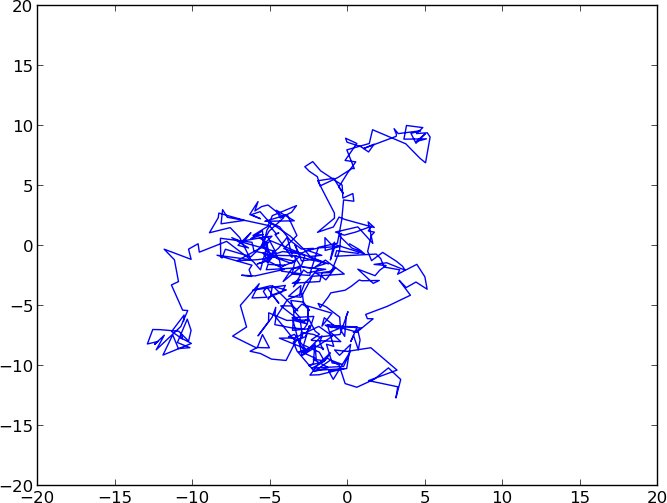
\includegraphics[width=0.8\textwidth]{one_particle.jpg}
% 
%     \end{columns}
% 
%     \bigskip
%     \bigskip
% 
%     Monte Carlo - Random walk (no interaction)
%     \begin{align*}
%         R_{x,i}(t+dt) = R_{x,i}(t) + \mathrm{random()}\\
%         R_{y,i}(t+dt) = R_{y,i}(t) + \mathrm{random()}
%     \end{align*}
% 
% \end{frame}


% \begin{frame}[fragile]
% 
%     \frametitle{Diffusion}
% 
%     Fick's second law of diffusion
%     \begin{align*}
%         \frac{\partial \phi }{\partial t} = D \frac{\partial^2 \phi }{\partial x^2}
%     \end{align*}
% 
%     Solution: a gauss-function
%     \begin{align*}
%         \phi(x, t) = \frac{1}{\sqrt{2 \pi \sigma^2}} \exp \left (-\frac{x^2}{2 \sigma^2} \right )
%     \end{align*}
% 
%     \begin{itemize}
%         \item $\sigma = \sqrt{2 D t}$ or $D = \sigma^2/2t$
%         \item in 3 dimensions, $x^2$ becomes $x^2 + y^2 + z^2$
%     \end{itemize}
% 
%     if we can simulate $\phi(x,t)$ we can calculate $D$.
% 
% \end{frame}
% 

\begin{frame}[fragile]

    \frametitle{The exercise, in Numpy}

    Velo-Verlet, Update positions, the Numpy way
    \begin{align*}
        R_x(t + dt) = R_x(t) + dt\ V_x(t) + 0.5\ dt^2\ A_x(t) \label{eq:position_x}
    \end{align*}


    \bigskip

\begin{lstlisting}
for n in range(n_steps):
    for i in range(n_particles):
        X[i] = X[i] + dt*Vx[i] + 0.5*dt*dt*Fx[i]
\end{lstlisting}

becomes

\begin{lstlisting}
for n in range(n_steps):
    X += dt*Vx + 0.5*dt*dt*Fx
\end{lstlisting}

\end{frame}






%%%%%%%%%%%%%%%%%%%%%%%%%%%%%%%%%%%%%%%%%%%%%%%%%%%%%%%%%%%%%%%%%%%%%%
%% END FRAMES
%%%%%%%%%%%%%%%%%%%%%%%%%%%%%%%%%%%%%%%%%%%%%%%%%%%%%%%%%%%%%%%%%%%%%%

\end{document}

